\section{\ref{PS:Q:Scalability}}

\textit{Will the regulation cycle time of the new decentralized solution scale better than the current Siemens system in terms of number of turbines per Park Pilot?}\newline\newline

\noindent As mentioned in \cref{cha:existingSystem} the centralized solution is a simulation of the current Siemens system. Thus to complete the comparison between the decentralized solution and the current Siemens system, the discussion section of this experiment also contains a discussion with regards to differences between the centralized solution and the current Siemens system (described in \cref{sec:CenAndCurrentSiemensSystemComparison}).

\subsection{Experiment}
\label{subsec:Exper:Scale}

The \ref{PS:Q:Scalability} problem asks for a comparison between the decentralized solution and the current Siemens system, in order to determine which of the systems scales best, in terms of decreasing the coupling between the regulation cycle time and the number of turbines. For this experiment we compare the results of the \ref{PS:Q:Performance} problem with acquired results from the centralized solution. Thus for this comparison, we study how the regulation cycle time changes when increasing the number of turbines for both systems.


\begin{figure}[b]
	%The figure show how regulation time differs central vs decantral
	\centering
	{\sffamily{Centralized approach}}
	\newline
	

{ %The brackets issolate the enviroment

\makeatletter
\ifcsname c@wavenum\endcsname %Only create one counter
\else
	\newcounter{wavenum}
\fi
\makeatother

\newcommand*{\bitvector}[3]{
  \draw[fill=#3] (t_cur) -- ++( .1, .3) -- ++(#2-.2,0) -- ++(.1, -.3)
                         -- ++(-.1,-.3) -- ++(.2-#2,0) -- cycle;
  \path (t_cur) -- node[anchor=mid] {#1} ++(#2,0) node[time] (t_cur) {};
}

% \known{val}{length}
\newcommand*{\known}[2]{
    \bitvector{#1}{#2}{white}
}

% \unknown{length}
\newcommand*{\unknown}[2]{
    \bitvector{#1}{#2}{black!20}
}

% \nextwave{name}
\newcommand{\nextwave}[1]{
  \path (0,\value{wavenum}) node[left] {#1} node[time] (t_cur) {};
  \addtocounter{wavenum}{-1}
}

% \begin{wave}[clkname]{num_waves}{clock_cycles}
\newenvironment{wave}{
  \begin{tikzpicture}[draw=black, yscale=.8,xscale=1]
    \tikzstyle{time}=[coordinate]
    \setlength{\unitlength}{1cm}
    \setcounter{wavenum}{0}
    
}{\end{tikzpicture}}

%%% End of timing.sty

\begin{wave}
 \nextwave{Regulation Time} \unknown{SendData}{2} \known{WaitForData}{5} \unknown{ReciveData}{2} \unknown{Calculate}{2}
\end{wave}
}

	\newline
	
	{\sffamily{Decentralized approach with seperate data reception}}
	

{ %The brackets issolate the enviroment

\makeatletter
\ifcsname c@wavenum\endcsname %Only create one counter
\else
	\newcounter{wavenum}
\fi
\makeatother

\newcommand*{\bitvector}[3]{
  \draw[fill=#3] (t_cur) -- ++( .1, .3) -- ++(#2-.2,0) -- ++(.1, -.3)
                         -- ++(-.1,-.3) -- ++(.2-#2,0) -- cycle;
  \path (t_cur) -- node[anchor=mid](textNode) {#1} ++(#2,0) node[time] (t_cur) {};
}

% \known{val}{length}
\newcommand*{\known}[2]{
    \bitvector{#1}{#2}{white}
}

% \unknown{length}
\newcommand*{\unknown}[2]{
    \bitvector{#1}{#2}{black!20}
}

% \nextwave{name}
\newcommand{\nextwave}[1]{
  %\path (0,\value{wavenum}) node[left] {#1} node[time] (t_cur) {};
  \path (0,\value{wavenum}) node[time] (t_cur) {};
  \addtocounter{wavenum}{-1}
}

%\newcommand{\timeSpanLabel}{
%	\node (CycleTimeLabel) [rectangle, above = 0.25cm of textNode, inner sep=10pt] {CycleTime};	  
%}

\newcommand{\timeSpanLabel}{
	\node (CycleTimeLabel) [rectangle, above = 1.02cm of t_cur, inner sep=0pt] {Regulation cycle time};
}

\newcommand{\timeSpanA}{
	\node (t_timeSpanA) [point, above = 0 of t_cur] {};	  
}

\newcommand{\timeSpanB}{
	\node (t_timeSpanB) [point, above =0 of t_cur] {};
	
	\graph[use existing nodes]{
		t_timeSpanA --[time span=1cm] CycleTimeLabel;
		CycleTimeLabel.south --[time span=-0.24cm] t_timeSpanB;
	}; 
	
}

%%% End of timing.sty

\begin{tikzpicture}[
	point/.style={inner sep=0pt}, %circle,minimum size=2pt,fill=red},
	draw=black, 
	yscale=.8,
	xscale=1,
	hv path/.style={to path={-| (\tikztotarget)}},
	vh path/.style={to path={|- (\tikztotarget)}},
	skip loop v/.style={to path={-- ++(#1,0) |- (\tikztotarget)}},		
	skip loop h/.style={to path={-- ++(0,#1) -| (\tikztotarget)}},
	time span/.style={to path={-- ++(0,#1) -| (\tikztotarget)}},
	graphs/every graph/.style={edges=rounded corners}	
]
	
\tikzstyle{time}=[coordinate]
\setlength{\unitlength}{1cm}
\setcounter{wavenum}{0}

	\nextwave{} \timeSpanA \unknown{readStates}{3} \unknown{calculate}{3} \timeSpanLabel \unknown{setSetpoint}{3} \unknown{sendState}{3} \timeSpanB \known{wait}{2}
	\nextwave{} \known{reciveStates}{14}
\end{tikzpicture}
}

	\caption{Centralized vs decentralized regulation time}
	\label{fig:timingCentralVSDecentral}
\end{figure}

The regulation cycle time of the decentralized solution is defined as the difference between the receive timestamp of the oldest turbine state (tOldestState) received and the timestamp sampled right after, a new turbine state has been sent (tSent):

$$regulation~cycle~time=tSent-tOldestState$$

The timestamp of the oldest turbine state is used to include network traffic in the regulation cycle time. Thus, if the decentralized solution is using cached data this will be reflected in the regulation cycle time, making the comparison between the centralized and decentralized solution more fair. 
%The aim is to compare the regulation cycle time including , therefore the turbine side centralized solution is not measured. This means that the decentralized version is at a slight disadvantage, since .

We use the following box plot type (for \cref{fig:exp:decen:sleep} and \cref{fig:exp:decen:turbines}): The central mark is the median, the edges of the box are the 25th and 75th percentiles, the whiskers extend to the most extreme data points not considered outliers, and outliers are plotted individually. The whisker length is denoted as 1.5 IQR. 

The following procedure is used each time the experiment is performed:

\begin{minipage}{\textwidth}
	\begin{enumerate}
		\item Start the system with N turbines.
		\item Make sure the system is stable.
		\item Start logging regulation cycle time.
		\item Stop logging after \experiemntRunTime.
		\end{enumerate}
\end{minipage}


\subsection{Results}

\begin{figure}[h!]
	\centering
%	\begin{tikzpicture}
\begin{axis}
[
	width=\resultsPlotWidthScale\textwidth,
	axis y line*=left,
	xlabel=Number of turbines,
	ylabel=Regulation cycle time (ms),
	ymin = 0,
	xmin = 1, xmax = 20,
	xtick={1, 2, 3, 4, 5, 6, 7, 8, 9, 10, 11, 12, 13, 14, 15, 16, 17, 18, 19},
	xticklabels={ , , 15, , 25, , 35, , 45, , 55, , 65, , 75, , 85, , 95},
%	xticklabels={5, 10, 15, 20, 25, 30, 35, 40, 45, 50, 55, 60, 65, 70, 75, 80, 85, 90, 95},
	boxplot/draw direction=y,
	ymajorgrids=true,
	yminorgrids=true,
%	minor y tick num=1,
	max space between ticks=17.5
]

%% /home/stefan/work/TestResults/Test4_Centralized_success_12-4-2014_2024/CentralizedLog2.csv
%\buildBoxPlot{0.871522}{0.955}{0.809034}{12.535623}{0.541744}
\buildBoxPlot[black]{0}{0}{0}{0}{0}

%% /home/stefan/work/TestResults/Test4_Centralized_success_12-4-2014_2024/CentralizedLog3.csv
\buildBoxPlot{1.168815}{1.310873}{1.081427}{24.566027}{0.591135}

%% /home/stefan/work/TestResults/Test4_Centralized_success_12-4-2014_2024/CentralizedLog4.csv
\buildBoxPlot{1.398871}{1.613768}{1.303639}{19.188073}{0.747894}

%% /home/stefan/work/TestResults/Test4_Centralized_success_12-4-2014_2024/CentralizedLog5.csv
\buildBoxPlot{1.722236}{1.981776}{1.596331}{13.257023}{1.077214}

%% /home/stefan/work/TestResults/Test4_Centralized_success_12-4-2014_2024/CentralizedLog6.csv
\buildBoxPlot{1.978881}{2.337657}{1.823133}{20.243534}{1.278172}

%% /home/stefan/work/TestResults/Test4_Centralized_success_12-4-2014_2024/CentralizedLog7.csv
\buildBoxPlot{2.985681}{3.527133}{2.724617}{102.89112}{1.917354}

%% /home/stefan/work/TestResults/Test4_Centralized_success_12-4-2014_2024/CentralizedLog8.csv
\buildBoxPlot{5.662268}{6.776311}{5.315074}{55.800126}{3.845115}

%% /home/stefan/work/TestResults/Test4_Centralized_success_12-4-2014_2024/CentralizedLog9.csv
\buildBoxPlot{14.607313}{22.842589}{10.21933}{40.119104}{7.578863}

%% /home/stefan/work/TestResults/Test4_Centralized_success_12-4-2014_2024/CentralizedLog10.csv
\buildBoxPlot{16.673738}{25.382756}{14.810635}{46.844742}{12.042462}

%% /home/stefan/work/TestResults/Test4_Centralized_success_12-4-2014_2024/CentralizedLog11.csv
\buildBoxPlot{20.220936}{27.962488}{19.190067}{63.348974}{17.058657}

%% /home/stefan/work/TestResults/Test4_Centralized_success_12-4-2014_2024/CentralizedLog12.csv
\buildBoxPlot{31.587407}{33.177592}{24.950794}{46.841843}{22.941051}

%% /home/stefan/work/TestResults/Test4_Centralized_success_12-4-2014_2024/CentralizedLog13.csv
\buildBoxPlot{36.93711}{38.790125}{32.230331}{51.398495}{29.702809}

%% /home/stefan/work/TestResults/Test4_Centralized_success_12-4-2014_2024/CentralizedLog14.csv
\buildBoxPlot{40.231022}{42.885333}{36.673407}{77.051599}{33.854906}

%% /home/stefan/work/TestResults/Test4_Centralized_success_12-4-2014_2024/CentralizedLog15.csv
\buildBoxPlot{45.380062}{48.694656}{42.841453}{225.894089}{39.402015}

%% /home/stefan/work/TestResults/Test4_Centralized_success_12-4-2014_2024/CentralizedLog16.csv
\buildBoxPlot{51.425649}{54.462315}{48.438981}{250.200229}{45.062697}

%% /home/stefan/work/TestResults/Test4_Centralized_success_12-4-2014_2024/CentralizedLog17.csv
\buildBoxPlot{58.196177}{62.557505}{55.582236}{271.626595}{51.598593}

%% /home/stefan/work/TestResults/Test4_Centralized_success_12-4-2014_2024/CentralizedLog18.csv
\buildBoxPlot{64.70376}{70.553035}{62.053219}{278.866888}{57.401402}

%% /home/stefan/work/TestResults/Test4_Centralized_success_12-4-2014_2024/CentralizedLog19.csv
\buildBoxPlot{73.715686}{80.566923}{69.809765}{287.542878}{65.698499}

%% /home/stefan/work/TestResults/Test4_Centralized_success_12-4-2014_2024/CentralizedLog20.csv
\buildBoxPlot{82.961949}{151.608592}{77.825807}{290.243704}{72.589561}


\addplot[thick, red!70] coordinates {
%	(1 ,0.871522)
	(2 ,1.168815)
	(3 ,1.398871)
	(4 ,1.722236)
	(5 ,1.978881)
	(6 ,2.985681)
	(7 ,5.662268)
	(8 ,14.607313)
	(9 ,16.673738)
	(10 ,20.220936)
	(11 ,31.587407)
	(12 ,36.93711)
	(13 ,40.231022)
	(14 ,45.380062)
	(15 ,51.425649)
	(16 ,58.196177)
	(17 ,64.70376)
	(18 ,73.715686)
	(19 ,82.961949)
};

\end{axis}
\end{tikzpicture}

%	% This file was created by matlab2tikz.
% Minimal pgfplots version: 1.3
%
%The latest updates can be retrieved from
%  http://www.mathworks.com/matlabcentral/fileexchange/22022-matlab2tikz
%where you can also make suggestions and rate matlab2tikz.
%
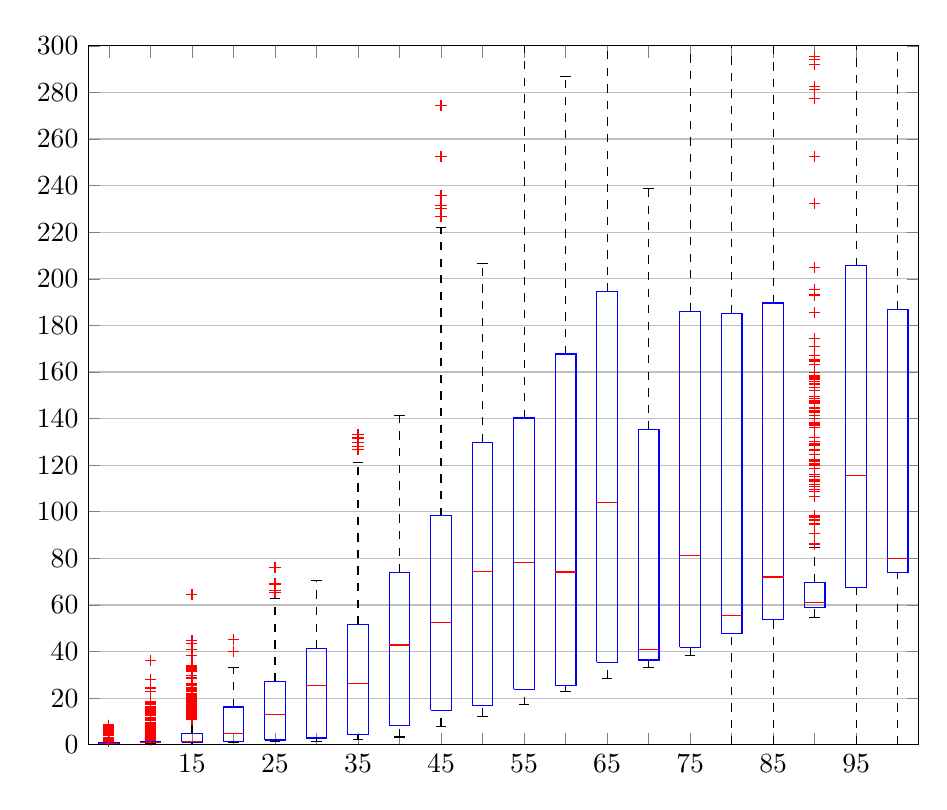
\begin{tikzpicture}

\begin{axis}[%
	width=\resultsPlotWidthScale\textwidth,
	xmin=0.5,
	xmax=20.5,
	xtick={1, 2, 3, 4, 5, 6, 7, 8, 9, 10, 11, 12, 13, 14, 15, 16, 17, 18, 19},
	xticklabels={ , , 15, , 25, , 35, , 45, , 55, , 65, , 75, , 85, , 95},
	ymin=0,
	ymax=300,
	ymajorgrids=true,
	yminorgrids=true,
	max space between ticks=17.5
]
\addplot [color=black,dashed,forget plot]
  table[row sep=crcr]{%
1	0.8717095\\
1	1.204627\\
};
\addplot [color=black,dashed,forget plot]
  table[row sep=crcr]{%
2	1.2604475\\
2	1.888937\\
};
\addplot [color=black,dashed,forget plot]
  table[row sep=crcr]{%
3	4.944662\\
3	10.675016\\
};
\addplot [color=black,dashed,forget plot]
  table[row sep=crcr]{%
4	16.2032205\\
4	33.311733\\
};
\addplot [color=black,dashed,forget plot]
  table[row sep=crcr]{%
5	27.053618\\
5	62.899558\\
};
\addplot [color=black,dashed,forget plot]
  table[row sep=crcr]{%
6	41.2910465\\
6	70.350287\\
};
\addplot [color=black,dashed,forget plot]
  table[row sep=crcr]{%
7	51.581584\\
7	121.085436\\
};
\addplot [color=black,dashed,forget plot]
  table[row sep=crcr]{%
8	73.910551\\
8	141.135822\\
};
\addplot [color=black,dashed,forget plot]
  table[row sep=crcr]{%
9	98.232932\\
9	222.18631\\
};
\addplot [color=black,dashed,forget plot]
  table[row sep=crcr]{%
10	129.9151\\
10	206.701738\\
};
\addplot [color=black,dashed,forget plot]
  table[row sep=crcr]{%
11	140.2385985\\
11	307.003647\\
};
\addplot [color=black,dashed,forget plot]
  table[row sep=crcr]{%
12	167.7148685\\
12	286.824347\\
};
\addplot [color=black,dashed,forget plot]
  table[row sep=crcr]{%
13	194.42233\\
13	426.984091\\
};
\addplot [color=black,dashed,forget plot]
  table[row sep=crcr]{%
14	135.221256\\
14	238.898358\\
};
\addplot [color=black,dashed,forget plot]
  table[row sep=crcr]{%
15	185.872368\\
15	399.208961\\
};
\addplot [color=black,dashed,forget plot]
  table[row sep=crcr]{%
16	185.049093\\
16	387.933056\\
};
\addplot [color=black,dashed,forget plot]
  table[row sep=crcr]{%
17	189.620724\\
17	390.403391\\
};
\addplot [color=black,dashed,forget plot]
  table[row sep=crcr]{%
18	69.756227\\
18	84.575222\\
};
\addplot [color=black,dashed,forget plot]
  table[row sep=crcr]{%
19	205.557893\\
19	412.155966\\
};
\addplot [color=black,dashed,forget plot]
  table[row sep=crcr]{%
20	186.7835205\\
20	355.119078\\
};
\addplot [color=black,dashed,forget plot]
  table[row sep=crcr]{%
1	0.452249\\
1	0.6489595\\
};
\addplot [color=black,dashed,forget plot]
  table[row sep=crcr]{%
2	0.604707\\
2	0.8393005\\
};
\addplot [color=black,dashed,forget plot]
  table[row sep=crcr]{%
3	0\\
3	1.1243275\\
};
\addplot [color=black,dashed,forget plot]
  table[row sep=crcr]{%
4	1.021879\\
4	1.5244415\\
};
\addplot [color=black,dashed,forget plot]
  table[row sep=crcr]{%
5	1.244611\\
5	2.061173\\
};
\addplot [color=black,dashed,forget plot]
  table[row sep=crcr]{%
6	1.524188\\
6	2.90871\\
};
\addplot [color=black,dashed,forget plot]
  table[row sep=crcr]{%
7	2.156496\\
7	4.2507545\\
};
\addplot [color=black,dashed,forget plot]
  table[row sep=crcr]{%
8	3.330849\\
8	8.282937\\
};
\addplot [color=black,dashed,forget plot]
  table[row sep=crcr]{%
9	7.831812\\
9	14.81487\\
};
\addplot [color=black,dashed,forget plot]
  table[row sep=crcr]{%
10	12.246399\\
10	16.6843555\\
};
\addplot [color=black,dashed,forget plot]
  table[row sep=crcr]{%
11	17.135656\\
11	23.771084\\
};
\addplot [color=black,dashed,forget plot]
  table[row sep=crcr]{%
12	22.778828\\
12	25.513819\\
};
\addplot [color=black,dashed,forget plot]
  table[row sep=crcr]{%
13	28.467515\\
13	35.4142585\\
};
\addplot [color=black,dashed,forget plot]
  table[row sep=crcr]{%
14	33.316406\\
14	36.380356\\
};
\addplot [color=black,dashed,forget plot]
  table[row sep=crcr]{%
15	38.153571\\
15	41.905524\\
};
\addplot [color=black,dashed,forget plot]
  table[row sep=crcr]{%
16	0\\
16	47.5835365\\
};
\addplot [color=black,dashed,forget plot]
  table[row sep=crcr]{%
17	0\\
17	53.6428275\\
};
\addplot [color=black,dashed,forget plot]
  table[row sep=crcr]{%
18	54.565993\\
18	58.849282\\
};
\addplot [color=black,dashed,forget plot]
  table[row sep=crcr]{%
19	0\\
19	67.47031\\
};
\addplot [color=black,dashed,forget plot]
  table[row sep=crcr]{%
20	0\\
20	74.0472365\\
};
\addplot [color=black,solid,forget plot]
  table[row sep=crcr]{%
0.875	1.204627\\
1.125	1.204627\\
};
\addplot [color=black,solid,forget plot]
  table[row sep=crcr]{%
1.875	1.888937\\
2.125	1.888937\\
};
\addplot [color=black,solid,forget plot]
  table[row sep=crcr]{%
2.875	10.675016\\
3.125	10.675016\\
};
\addplot [color=black,solid,forget plot]
  table[row sep=crcr]{%
3.875	33.311733\\
4.125	33.311733\\
};
\addplot [color=black,solid,forget plot]
  table[row sep=crcr]{%
4.875	62.899558\\
5.125	62.899558\\
};
\addplot [color=black,solid,forget plot]
  table[row sep=crcr]{%
5.875	70.350287\\
6.125	70.350287\\
};
\addplot [color=black,solid,forget plot]
  table[row sep=crcr]{%
6.875	121.085436\\
7.125	121.085436\\
};
\addplot [color=black,solid,forget plot]
  table[row sep=crcr]{%
7.875	141.135822\\
8.125	141.135822\\
};
\addplot [color=black,solid,forget plot]
  table[row sep=crcr]{%
8.875	222.18631\\
9.125	222.18631\\
};
\addplot [color=black,solid,forget plot]
  table[row sep=crcr]{%
9.875	206.701738\\
10.125	206.701738\\
};
\addplot [color=black,solid,forget plot]
  table[row sep=crcr]{%
10.875	307.003647\\
11.125	307.003647\\
};
\addplot [color=black,solid,forget plot]
  table[row sep=crcr]{%
11.875	286.824347\\
12.125	286.824347\\
};
\addplot [color=black,solid,forget plot]
  table[row sep=crcr]{%
12.875	426.984091\\
13.125	426.984091\\
};
\addplot [color=black,solid,forget plot]
  table[row sep=crcr]{%
13.875	238.898358\\
14.125	238.898358\\
};
\addplot [color=black,solid,forget plot]
  table[row sep=crcr]{%
14.875	399.208961\\
15.125	399.208961\\
};
\addplot [color=black,solid,forget plot]
  table[row sep=crcr]{%
15.875	387.933056\\
16.125	387.933056\\
};
\addplot [color=black,solid,forget plot]
  table[row sep=crcr]{%
16.875	390.403391\\
17.125	390.403391\\
};
\addplot [color=black,solid,forget plot]
  table[row sep=crcr]{%
17.875	84.575222\\
18.125	84.575222\\
};
\addplot [color=black,solid,forget plot]
  table[row sep=crcr]{%
18.875	412.155966\\
19.125	412.155966\\
};
\addplot [color=black,solid,forget plot]
  table[row sep=crcr]{%
19.875	355.119078\\
20.125	355.119078\\
};
\addplot [color=black,solid,forget plot]
  table[row sep=crcr]{%
0.875	0.452249\\
1.125	0.452249\\
};
\addplot [color=black,solid,forget plot]
  table[row sep=crcr]{%
1.875	0.604707\\
2.125	0.604707\\
};
\addplot [color=black,solid,forget plot]
  table[row sep=crcr]{%
2.875	0\\
3.125	0\\
};
\addplot [color=black,solid,forget plot]
  table[row sep=crcr]{%
3.875	1.021879\\
4.125	1.021879\\
};
\addplot [color=black,solid,forget plot]
  table[row sep=crcr]{%
4.875	1.244611\\
5.125	1.244611\\
};
\addplot [color=black,solid,forget plot]
  table[row sep=crcr]{%
5.875	1.524188\\
6.125	1.524188\\
};
\addplot [color=black,solid,forget plot]
  table[row sep=crcr]{%
6.875	2.156496\\
7.125	2.156496\\
};
\addplot [color=black,solid,forget plot]
  table[row sep=crcr]{%
7.875	3.330849\\
8.125	3.330849\\
};
\addplot [color=black,solid,forget plot]
  table[row sep=crcr]{%
8.875	7.831812\\
9.125	7.831812\\
};
\addplot [color=black,solid,forget plot]
  table[row sep=crcr]{%
9.875	12.246399\\
10.125	12.246399\\
};
\addplot [color=black,solid,forget plot]
  table[row sep=crcr]{%
10.875	17.135656\\
11.125	17.135656\\
};
\addplot [color=black,solid,forget plot]
  table[row sep=crcr]{%
11.875	22.778828\\
12.125	22.778828\\
};
\addplot [color=black,solid,forget plot]
  table[row sep=crcr]{%
12.875	28.467515\\
13.125	28.467515\\
};
\addplot [color=black,solid,forget plot]
  table[row sep=crcr]{%
13.875	33.316406\\
14.125	33.316406\\
};
\addplot [color=black,solid,forget plot]
  table[row sep=crcr]{%
14.875	38.153571\\
15.125	38.153571\\
};
\addplot [color=black,solid,forget plot]
  table[row sep=crcr]{%
15.875	0\\
16.125	0\\
};
\addplot [color=black,solid,forget plot]
  table[row sep=crcr]{%
16.875	0\\
17.125	0\\
};
\addplot [color=black,solid,forget plot]
  table[row sep=crcr]{%
17.875	54.565993\\
18.125	54.565993\\
};
\addplot [color=black,solid,forget plot]
  table[row sep=crcr]{%
18.875	0\\
19.125	0\\
};
\addplot [color=black,solid,forget plot]
  table[row sep=crcr]{%
19.875	0\\
20.125	0\\
};
\addplot [color=blue,solid,forget plot]
  table[row sep=crcr]{%
0.75	0.6489595\\
0.75	0.8717095\\
1.25	0.8717095\\
1.25	0.6489595\\
0.75	0.6489595\\
};
\addplot [color=blue,solid,forget plot]
  table[row sep=crcr]{%
1.75	0.8393005\\
1.75	1.2604475\\
2.25	1.2604475\\
2.25	0.8393005\\
1.75	0.8393005\\
};
\addplot [color=blue,solid,forget plot]
  table[row sep=crcr]{%
2.75	1.1243275\\
2.75	4.944662\\
3.25	4.944662\\
3.25	1.1243275\\
2.75	1.1243275\\
};
\addplot [color=blue,solid,forget plot]
  table[row sep=crcr]{%
3.75	1.5244415\\
3.75	16.2032205\\
4.25	16.2032205\\
4.25	1.5244415\\
3.75	1.5244415\\
};
\addplot [color=blue,solid,forget plot]
  table[row sep=crcr]{%
4.75	2.061173\\
4.75	27.053618\\
5.25	27.053618\\
5.25	2.061173\\
4.75	2.061173\\
};
\addplot [color=blue,solid,forget plot]
  table[row sep=crcr]{%
5.75	2.90871\\
5.75	41.2910465\\
6.25	41.2910465\\
6.25	2.90871\\
5.75	2.90871\\
};
\addplot [color=blue,solid,forget plot]
  table[row sep=crcr]{%
6.75	4.2507545\\
6.75	51.581584\\
7.25	51.581584\\
7.25	4.2507545\\
6.75	4.2507545\\
};
\addplot [color=blue,solid,forget plot]
  table[row sep=crcr]{%
7.75	8.282937\\
7.75	73.910551\\
8.25	73.910551\\
8.25	8.282937\\
7.75	8.282937\\
};
\addplot [color=blue,solid,forget plot]
  table[row sep=crcr]{%
8.75	14.81487\\
8.75	98.232932\\
9.25	98.232932\\
9.25	14.81487\\
8.75	14.81487\\
};
\addplot [color=blue,solid,forget plot]
  table[row sep=crcr]{%
9.75	16.6843555\\
9.75	129.9151\\
10.25	129.9151\\
10.25	16.6843555\\
9.75	16.6843555\\
};
\addplot [color=blue,solid,forget plot]
  table[row sep=crcr]{%
10.75	23.771084\\
10.75	140.2385985\\
11.25	140.2385985\\
11.25	23.771084\\
10.75	23.771084\\
};
\addplot [color=blue,solid,forget plot]
  table[row sep=crcr]{%
11.75	25.513819\\
11.75	167.7148685\\
12.25	167.7148685\\
12.25	25.513819\\
11.75	25.513819\\
};
\addplot [color=blue,solid,forget plot]
  table[row sep=crcr]{%
12.75	35.4142585\\
12.75	194.42233\\
13.25	194.42233\\
13.25	35.4142585\\
12.75	35.4142585\\
};
\addplot [color=blue,solid,forget plot]
  table[row sep=crcr]{%
13.75	36.380356\\
13.75	135.221256\\
14.25	135.221256\\
14.25	36.380356\\
13.75	36.380356\\
};
\addplot [color=blue,solid,forget plot]
  table[row sep=crcr]{%
14.75	41.905524\\
14.75	185.872368\\
15.25	185.872368\\
15.25	41.905524\\
14.75	41.905524\\
};
\addplot [color=blue,solid,forget plot]
  table[row sep=crcr]{%
15.75	47.5835365\\
15.75	185.049093\\
16.25	185.049093\\
16.25	47.5835365\\
15.75	47.5835365\\
};
\addplot [color=blue,solid,forget plot]
  table[row sep=crcr]{%
16.75	53.6428275\\
16.75	189.620724\\
17.25	189.620724\\
17.25	53.6428275\\
16.75	53.6428275\\
};
\addplot [color=blue,solid,forget plot]
  table[row sep=crcr]{%
17.75	58.849282\\
17.75	69.756227\\
18.25	69.756227\\
18.25	58.849282\\
17.75	58.849282\\
};
\addplot [color=blue,solid,forget plot]
  table[row sep=crcr]{%
18.75	67.47031\\
18.75	205.557893\\
19.25	205.557893\\
19.25	67.47031\\
18.75	67.47031\\
};
\addplot [color=blue,solid,forget plot]
  table[row sep=crcr]{%
19.75	74.0472365\\
19.75	186.7835205\\
20.25	186.7835205\\
20.25	74.0472365\\
19.75	74.0472365\\
};
\addplot [color=red,solid,forget plot]
  table[row sep=crcr]{%
0.75	0.727033\\
1.25	0.727033\\
};
\addplot [color=red,solid,forget plot]
  table[row sep=crcr]{%
1.75	0.9325085\\
2.25	0.9325085\\
};
\addplot [color=red,solid,forget plot]
  table[row sep=crcr]{%
2.75	1.3743515\\
3.25	1.3743515\\
};
\addplot [color=red,solid,forget plot]
  table[row sep=crcr]{%
3.75	4.791979\\
4.25	4.791979\\
};
\addplot [color=red,solid,forget plot]
  table[row sep=crcr]{%
4.75	13.090375\\
5.25	13.090375\\
};
\addplot [color=red,solid,forget plot]
  table[row sep=crcr]{%
5.75	25.5858225\\
6.25	25.5858225\\
};
\addplot [color=red,solid,forget plot]
  table[row sep=crcr]{%
6.75	26.3139895\\
7.25	26.3139895\\
};
\addplot [color=red,solid,forget plot]
  table[row sep=crcr]{%
7.75	42.7994295\\
8.25	42.7994295\\
};
\addplot [color=red,solid,forget plot]
  table[row sep=crcr]{%
8.75	52.370321\\
9.25	52.370321\\
};
\addplot [color=red,solid,forget plot]
  table[row sep=crcr]{%
9.75	74.509338\\
10.25	74.509338\\
};
\addplot [color=red,solid,forget plot]
  table[row sep=crcr]{%
10.75	78.4097345\\
11.25	78.4097345\\
};
\addplot [color=red,solid,forget plot]
  table[row sep=crcr]{%
11.75	74.1398775\\
12.25	74.1398775\\
};
\addplot [color=red,solid,forget plot]
  table[row sep=crcr]{%
12.75	103.919405\\
13.25	103.919405\\
};
\addplot [color=red,solid,forget plot]
  table[row sep=crcr]{%
13.75	40.8226565\\
14.25	40.8226565\\
};
\addplot [color=red,solid,forget plot]
  table[row sep=crcr]{%
14.75	81.151909\\
15.25	81.151909\\
};
\addplot [color=red,solid,forget plot]
  table[row sep=crcr]{%
15.75	55.4174655\\
16.25	55.4174655\\
};
\addplot [color=red,solid,forget plot]
  table[row sep=crcr]{%
16.75	71.9904755\\
17.25	71.9904755\\
};
\addplot [color=red,solid,forget plot]
  table[row sep=crcr]{%
17.75	60.9902745\\
18.25	60.9902745\\
};
\addplot [color=red,solid,forget plot]
  table[row sep=crcr]{%
18.75	115.484537\\
19.25	115.484537\\
};
\addplot [color=red,solid,forget plot]
  table[row sep=crcr]{%
19.75	79.967163\\
20.25	79.967163\\
};
\addplot [color=blue,only marks,mark=+,mark options={solid,draw=red},forget plot]
  table[row sep=crcr]{%
1	1.22142\\
1	1.223364\\
1	1.224134\\
1	1.233426\\
1	1.238923\\
1	1.249099\\
1	1.267809\\
1	1.284091\\
1	1.291981\\
1	1.319801\\
1	1.336661\\
1	1.415403\\
1	1.421902\\
1	1.503776\\
1	1.51294\\
1	1.532207\\
1	1.546875\\
1	1.547268\\
1	1.584143\\
1	1.589388\\
1	1.638589\\
1	1.811361\\
1	1.830223\\
1	1.831018\\
1	1.831122\\
1	1.835368\\
1	1.844371\\
1	2.105473\\
1	2.236183\\
1	2.251674\\
1	2.280143\\
1	2.299661\\
1	2.522178\\
1	2.750071\\
1	2.792578\\
1	3.25494\\
1	3.2941\\
1	3.929381\\
1	3.990809\\
1	4.137583\\
1	4.472371\\
1	4.537438\\
1	5.003565\\
1	5.006466\\
1	5.080215\\
1	5.089503\\
1	5.200881\\
1	5.250616\\
1	5.546884\\
1	5.625184\\
1	5.774674\\
1	5.797138\\
1	5.85168\\
1	5.899315\\
1	6.016238\\
1	6.033693\\
1	6.065686\\
1	6.074834\\
1	6.090889\\
1	6.127169\\
1	6.155085\\
1	6.426519\\
1	6.448381\\
1	6.519414\\
1	6.550741\\
1	6.582032\\
1	6.600282\\
1	6.737918\\
1	6.745443\\
1	6.750611\\
1	6.789309\\
1	6.798253\\
1	6.822493\\
1	6.995045\\
1	7.029346\\
1	7.053232\\
1	7.064158\\
1	7.07522\\
1	7.135983\\
1	7.160974\\
1	7.188216\\
1	7.222805\\
1	7.233565\\
1	7.249176\\
1	7.249689\\
1	7.27116\\
1	7.325184\\
1	7.352011\\
1	7.389161\\
1	7.426482\\
1	7.431757\\
1	7.463729\\
1	7.47152\\
1	7.522566\\
1	7.535727\\
1	7.545131\\
1	7.574998\\
1	7.635756\\
1	7.637039\\
1	7.681288\\
1	7.69941\\
1	7.713476\\
1	7.746304\\
1	7.80394\\
1	7.820249\\
1	7.866035\\
1	7.880942\\
1	7.974198\\
1	7.996921\\
1	8.016012\\
1	8.038029\\
1	8.038785\\
1	8.043832\\
1	8.054257\\
1	8.068841\\
1	8.094754\\
1	8.09828\\
1	8.100322\\
1	8.14914\\
1	8.165973\\
1	8.168417\\
1	8.197402\\
1	8.204572\\
1	8.211569\\
1	8.273737\\
1	8.292364\\
1	8.31482\\
1	8.323623\\
1	8.324661\\
1	8.35753\\
1	8.36441\\
1	8.443329\\
1	8.458258\\
};
\addplot [color=blue,only marks,mark=+,mark options={solid,draw=red},forget plot]
  table[row sep=crcr]{%
2	1.90167\\
2	1.911317\\
2	1.962956\\
2	1.968191\\
2	1.985629\\
2	1.990298\\
2	1.99821\\
2	1.999762\\
2	2.006972\\
2	2.01125\\
2	2.016703\\
2	2.060781\\
2	2.078726\\
2	2.084904\\
2	2.0886\\
2	2.149672\\
2	2.152386\\
2	2.157416\\
2	2.172206\\
2	2.210438\\
2	2.211897\\
2	2.265665\\
2	2.319203\\
2	2.320914\\
2	2.349612\\
2	2.398934\\
2	2.415953\\
2	2.462345\\
2	2.517542\\
2	2.518407\\
2	2.522352\\
2	2.559802\\
2	2.55986\\
2	2.588216\\
2	2.616982\\
2	2.640217\\
2	2.728957\\
2	2.763691\\
2	2.781829\\
2	2.796268\\
2	2.805757\\
2	2.809971\\
2	2.835864\\
2	2.857655\\
2	2.898538\\
2	2.902265\\
2	2.93052\\
2	2.958764\\
2	2.970508\\
2	2.981127\\
2	2.987679\\
2	2.993292\\
2	2.996044\\
2	3.003311\\
2	3.040946\\
2	3.044832\\
2	3.159759\\
2	3.171292\\
2	3.19803\\
2	3.223353\\
2	3.282729\\
2	3.322616\\
2	3.368547\\
2	3.522944\\
2	3.548358\\
2	3.57788\\
2	3.588871\\
2	3.709183\\
2	3.753555\\
2	4.156216\\
2	4.158493\\
2	4.17583\\
2	4.215829\\
2	4.22159\\
2	4.303591\\
2	4.378721\\
2	4.432432\\
2	4.496267\\
2	4.535655\\
2	4.562851\\
2	4.603645\\
2	4.626893\\
2	4.675847\\
2	4.697096\\
2	4.700302\\
2	4.704188\\
2	4.712042\\
2	4.793507\\
2	4.815152\\
2	4.857104\\
2	4.903281\\
2	4.925399\\
2	4.947763\\
2	5.141249\\
2	5.193353\\
2	5.338926\\
2	5.457376\\
2	5.767504\\
2	5.946886\\
2	6.065162\\
2	6.27828\\
2	6.380513\\
2	6.388238\\
2	6.414966\\
2	6.488282\\
2	6.659254\\
2	6.683566\\
2	6.877373\\
2	6.964909\\
2	7.118723\\
2	7.150523\\
2	7.184356\\
2	7.355692\\
2	7.373073\\
2	7.375065\\
2	7.387138\\
2	7.610728\\
2	7.827468\\
2	7.997416\\
2	8.003218\\
2	8.194986\\
2	8.875918\\
2	9.030813\\
2	9.168052\\
2	9.234478\\
2	9.240843\\
2	9.32023\\
2	9.355343\\
2	9.585629\\
2	9.632804\\
2	10.256122\\
2	10.54318\\
2	10.803498\\
2	10.849408\\
2	10.856044\\
2	10.946935\\
2	11.105923\\
2	11.112722\\
2	11.34085\\
2	11.612397\\
2	11.670481\\
2	11.712875\\
2	12.553934\\
2	12.558786\\
2	12.600901\\
2	12.730505\\
2	13.03436\\
2	13.59391\\
2	13.644562\\
2	14.067884\\
2	14.353523\\
2	14.417325\\
2	14.694076\\
2	14.763316\\
2	14.969792\\
2	14.992874\\
2	15.324704\\
2	15.355964\\
2	15.496052\\
2	15.989522\\
2	16.258874\\
2	16.543165\\
2	17.449576\\
2	17.943462\\
2	18.002392\\
2	18.307749\\
2	18.434977\\
2	22.673764\\
2	22.875711\\
2	24.368586\\
2	28.112777\\
2	36.326413\\
};
\addplot [color=blue,only marks,mark=+,mark options={solid,draw=red},forget plot]
  table[row sep=crcr]{%
3	10.712372\\
3	10.72463\\
3	10.824215\\
3	10.912497\\
3	10.934032\\
3	10.970966\\
3	11.133457\\
3	11.216931\\
3	11.239228\\
3	11.326209\\
3	11.337168\\
3	11.358172\\
3	11.440343\\
3	11.469403\\
3	11.51297\\
3	11.534249\\
3	11.610081\\
3	11.663412\\
3	11.694482\\
3	11.764268\\
3	11.788597\\
3	11.879232\\
3	11.88636\\
3	11.895998\\
3	11.951678\\
3	11.962575\\
3	12.136279\\
3	12.172993\\
3	12.18119\\
3	12.246693\\
3	12.301922\\
3	12.397148\\
3	12.649651\\
3	12.679065\\
3	12.736198\\
3	12.783409\\
3	12.846494\\
3	12.904049\\
3	12.983231\\
3	12.990299\\
3	12.999456\\
3	13.019261\\
3	13.133643\\
3	13.214978\\
3	13.294728\\
3	13.312276\\
3	13.361947\\
3	13.63175\\
3	13.636207\\
3	13.644932\\
3	13.834311\\
3	13.89846\\
3	13.935251\\
3	13.936967\\
3	13.984923\\
3	14.005203\\
3	14.066154\\
3	14.181378\\
3	14.216491\\
3	14.269401\\
3	14.371669\\
3	14.381037\\
3	14.391874\\
3	14.394386\\
3	14.406414\\
3	14.524739\\
3	14.653434\\
3	14.755178\\
3	14.874585\\
3	14.876075\\
3	15.017429\\
3	15.156781\\
3	15.305643\\
3	15.349046\\
3	15.516102\\
3	15.536637\\
3	15.593484\\
3	15.722859\\
3	16.133056\\
3	16.151682\\
3	16.251942\\
3	16.652387\\
3	16.82844\\
3	16.830175\\
3	16.845397\\
3	16.963685\\
3	17.027354\\
3	17.126082\\
3	17.175433\\
3	17.441423\\
3	17.447871\\
3	17.503013\\
3	18.054716\\
3	18.218939\\
3	18.232524\\
3	18.412774\\
3	18.471894\\
3	18.535344\\
3	18.547782\\
3	19.067263\\
3	19.288464\\
3	19.337552\\
3	19.550863\\
3	19.553737\\
3	19.65005\\
3	19.89144\\
3	20.004595\\
3	20.030844\\
3	20.076484\\
3	20.148205\\
3	20.24326\\
3	20.369406\\
3	20.548091\\
3	20.577104\\
3	20.989983\\
3	21.035488\\
3	21.265652\\
3	21.308726\\
3	21.391766\\
3	21.467402\\
3	21.487734\\
3	21.706475\\
3	21.806243\\
3	21.837835\\
3	21.847035\\
3	22.749871\\
3	23.003556\\
3	23.117597\\
3	23.162438\\
3	23.195855\\
3	23.466837\\
3	23.49557\\
3	23.627204\\
3	24.374648\\
3	24.422942\\
3	25.351046\\
3	25.782507\\
3	25.823924\\
3	25.873848\\
3	26.10141\\
3	26.481113\\
3	28.651801\\
3	28.687621\\
3	28.930998\\
3	29.6302\\
3	29.797236\\
3	31.334925\\
3	31.747665\\
3	32.48028\\
3	32.619401\\
3	33.017111\\
3	33.299365\\
3	33.710997\\
3	34.202288\\
3	38.391179\\
3	41.073174\\
3	43.384782\\
3	44.587852\\
3	44.822243\\
3	64.609355\\
};
\addplot [color=blue,only marks,mark=+,mark options={solid,draw=red},forget plot]
  table[row sep=crcr]{%
4	39.999706\\
4	45.044395\\
};
\addplot [color=blue,only marks,mark=+,mark options={solid,draw=red},forget plot]
  table[row sep=crcr]{%
5	65.437522\\
5	66.282007\\
5	68.917478\\
5	69.027589\\
5	69.32905\\
5	76.022717\\
};
\addplot [color=blue,only marks,mark=+,mark options={solid,draw=red},forget plot]
  table[row sep=crcr]{%
nan	nan\\
};
\addplot [color=blue,only marks,mark=+,mark options={solid,draw=red},forget plot]
  table[row sep=crcr]{%
7	126.57364\\
7	127.839887\\
7	129.633535\\
7	131.39321\\
7	131.744755\\
7	132.993896\\
};
\addplot [color=blue,only marks,mark=+,mark options={solid,draw=red},forget plot]
  table[row sep=crcr]{%
nan	nan\\
};
\addplot [color=blue,only marks,mark=+,mark options={solid,draw=red},forget plot]
  table[row sep=crcr]{%
9	226.846077\\
9	230.029879\\
9	231.330554\\
9	235.828114\\
9	252.531861\\
9	274.415257\\
};
\addplot [color=blue,only marks,mark=+,mark options={solid,draw=red},forget plot]
  table[row sep=crcr]{%
nan	nan\\
};
\addplot [color=blue,only marks,mark=+,mark options={solid,draw=red},forget plot]
  table[row sep=crcr]{%
11	328.644114\\
11	334.633811\\
11	347.48941\\
11	352.28358\\
};
\addplot [color=blue,only marks,mark=+,mark options={solid,draw=red},forget plot]
  table[row sep=crcr]{%
12	466.979415\\
12	790.974015\\
12	799.073064\\
12	807.138983\\
12	811.776466\\
12	825.995385\\
12	828.136598\\
12	828.636983\\
12	829.658051\\
12	830.027513\\
12	831.625153\\
12	860.149244\\
12	870.952407\\
12	925.896148\\
12	956.462884\\
12	980.212867\\
12	1475.832656\\
};
\addplot [color=blue,only marks,mark=+,mark options={solid,draw=red},forget plot]
  table[row sep=crcr]{%
13	436.452672\\
13	461.612621\\
13	464.72264\\
13	492.783547\\
};
\addplot [color=blue,only marks,mark=+,mark options={solid,draw=red},forget plot]
  table[row sep=crcr]{%
14	516.477803\\
14	521.131615\\
14	548.186438\\
14	553.249303\\
14	556.149607\\
14	574.576324\\
14	574.869284\\
14	577.742807\\
14	579.735296\\
14	584.686404\\
14	593.438547\\
14	596.380349\\
14	598.191485\\
14	598.84507\\
14	608.097375\\
14	617.101134\\
14	619.045276\\
14	619.953765\\
14	625.709395\\
14	629.279299\\
14	629.909969\\
14	637.550331\\
14	650.806984\\
14	655.873061\\
14	665.087489\\
14	668.713115\\
14	672.203926\\
14	674.734334\\
14	685.007391\\
14	685.276104\\
14	696.643168\\
14	702.755428\\
14	711.962523\\
14	713.90018\\
14	716.038134\\
14	717.987356\\
14	731.793634\\
14	732.812486\\
14	734.387525\\
14	735.553426\\
14	739.655719\\
14	741.138696\\
14	743.592059\\
14	749.511598\\
14	758.220628\\
14	767.173501\\
14	787.481231\\
14	791.741118\\
14	806.091296\\
14	807.148629\\
14	808.62873\\
14	813.961306\\
14	817.334614\\
14	817.433495\\
14	817.825926\\
14	820.848848\\
14	822.199013\\
14	827.34225\\
14	830.203037\\
14	830.9751\\
14	832.847263\\
14	834.140786\\
14	839.044581\\
14	845.966635\\
14	846.618104\\
14	854.936652\\
14	855.494969\\
14	859.374444\\
14	866.190171\\
14	870.842619\\
14	874.186476\\
14	883.121314\\
14	883.429961\\
14	885.89492\\
14	892.364938\\
14	895.886937\\
14	898.399519\\
14	900.917675\\
14	904.601228\\
14	919.104384\\
14	921.721725\\
14	923.317272\\
14	924.999961\\
14	929.178234\\
14	932.480675\\
14	938.552007\\
14	943.337044\\
14	947.603204\\
14	960.540944\\
14	961.402436\\
14	981.62104\\
14	981.970315\\
14	995.902458\\
14	998.546303\\
14	998.952993\\
14	1000.379985\\
14	1002.724105\\
14	1004.846879\\
14	1029.337594\\
14	1036.38101\\
14	1048.006164\\
14	1054.763013\\
14	1062.954368\\
14	1078.066665\\
14	1078.352514\\
14	1089.033734\\
14	1185.153126\\
14	1192.53254\\
};
\addplot [color=blue,only marks,mark=+,mark options={solid,draw=red},forget plot]
  table[row sep=crcr]{%
15	413.771069\\
15	415.537737\\
15	416.275727\\
15	416.638957\\
15	418.187265\\
15	429.650314\\
15	432.834924\\
15	436.729475\\
15	436.780207\\
15	447.391499\\
15	461.232542\\
15	468.187997\\
15	492.811488\\
};
\addplot [color=blue,only marks,mark=+,mark options={solid,draw=red},forget plot]
  table[row sep=crcr]{%
16	391.504739\\
16	393.266469\\
16	394.953183\\
16	400.079125\\
16	402.528077\\
16	402.59457\\
16	403.571968\\
16	404.604515\\
16	408.236184\\
16	410.786243\\
16	418.888676\\
16	421.719738\\
16	426.782423\\
16	429.928426\\
16	456.078929\\
16	456.144372\\
16	462.901035\\
16	466.222926\\
16	475.291873\\
16	494.781046\\
16	504.963081\\
16	512.937421\\
16	531.40812\\
16	537.32713\\
16	925.279886\\
};
\addplot [color=blue,only marks,mark=+,mark options={solid,draw=red},forget plot]
  table[row sep=crcr]{%
17	395.395536\\
17	396.185814\\
17	400.234754\\
17	400.919771\\
17	401.286572\\
17	401.44932\\
17	405.897657\\
17	406.550507\\
17	406.874901\\
17	409.850021\\
17	412.082702\\
17	412.29205\\
17	413.441619\\
17	418.860258\\
17	419.388793\\
17	420.870868\\
17	424.021534\\
17	425.802527\\
17	433.915915\\
17	434.473733\\
17	434.922242\\
17	435.478035\\
17	456.947733\\
17	460.611284\\
17	461.070377\\
17	467.248761\\
17	470.773971\\
17	474.641047\\
17	483.883285\\
17	488.567997\\
17	519.601736\\
17	529.774526\\
17	532.919833\\
17	541.579177\\
};
\addplot [color=blue,only marks,mark=+,mark options={solid,draw=red},forget plot]
  table[row sep=crcr]{%
18	86.159378\\
18	90.668505\\
18	94.440606\\
18	95.027982\\
18	96.177874\\
18	96.668815\\
18	97.51727\\
18	97.524343\\
18	97.961739\\
18	98.201713\\
18	106.504354\\
18	108.598272\\
18	109.386755\\
18	110.693345\\
18	111.61382\\
18	113.215588\\
18	113.998949\\
18	115.30506\\
18	116.084194\\
18	118.681951\\
18	119.784562\\
18	120.377811\\
18	120.539549\\
18	120.820783\\
18	121.687063\\
18	121.94637\\
18	122.404761\\
18	124.66292\\
18	126.255916\\
18	126.646287\\
18	128.615305\\
18	129.058219\\
18	129.308683\\
18	129.978064\\
18	130.146154\\
18	131.867658\\
18	136.250682\\
18	136.301259\\
18	136.915259\\
18	137.287311\\
18	137.924732\\
18	138.24477\\
18	138.363895\\
18	139.97497\\
18	141.274313\\
18	142.65381\\
18	142.785853\\
18	143.251243\\
18	144.273789\\
18	144.618031\\
18	144.701109\\
18	146.670355\\
18	147.314209\\
18	147.340368\\
18	147.720972\\
18	148.532556\\
18	149.467189\\
18	152.238227\\
18	153.168407\\
18	154.760433\\
18	154.964476\\
18	155.749014\\
18	155.98442\\
18	156.736876\\
18	156.750484\\
18	157.370718\\
18	157.404776\\
18	157.541901\\
18	157.872815\\
18	158.599972\\
18	159.809991\\
18	159.862686\\
18	163.176972\\
18	164.328241\\
18	165.034392\\
18	165.22673\\
18	167.233095\\
18	170.757205\\
18	174.316953\\
18	185.383809\\
18	192.887773\\
18	193.446229\\
18	195.274025\\
18	204.875554\\
18	232.269385\\
18	252.421417\\
18	277.39999\\
18	281.21265\\
18	282.571761\\
18	292.089637\\
18	294.003322\\
18	295.340114\\
18	306.445289\\
18	310.216001\\
18	316.22929\\
18	320.061372\\
18	330.890354\\
18	341.626899\\
18	343.59161\\
18	361.446167\\
18	363.177192\\
18	365.234394\\
18	366.878349\\
18	369.434197\\
18	370.667787\\
18	384.922705\\
18	385.597618\\
18	398.286229\\
18	401.356793\\
18	403.525193\\
18	414.925591\\
18	423.616652\\
18	430.152321\\
18	431.948109\\
18	432.166707\\
18	434.182315\\
18	435.375041\\
18	436.080741\\
18	437.833424\\
18	438.296088\\
18	447.623571\\
18	456.32524\\
18	463.234298\\
18	463.664204\\
18	466.356037\\
18	468.481474\\
18	476.083349\\
18	490.894297\\
18	495.430708\\
18	497.957675\\
18	510.218098\\
18	511.629683\\
18	518.204134\\
18	521.2447\\
18	524.646491\\
18	529.0453\\
18	548.305702\\
18	550.75314\\
18	556.834255\\
18	559.563867\\
18	560.999111\\
18	561.898571\\
18	563.805964\\
18	566.979079\\
18	569.477825\\
18	585.891429\\
18	593.081773\\
18	594.032478\\
18	598.754091\\
18	601.07898\\
18	603.136575\\
18	604.461436\\
18	606.685389\\
18	615.975934\\
18	620.809847\\
18	625.216047\\
18	630.588802\\
18	635.083585\\
18	642.385159\\
18	643.764533\\
18	644.34599\\
18	654.07332\\
18	655.095482\\
18	662.471484\\
18	672.075709\\
18	675.889961\\
18	678.529528\\
18	678.890173\\
18	679.892176\\
18	684.831434\\
18	693.301249\\
18	702.617589\\
18	704.800503\\
18	708.665208\\
18	708.977256\\
18	719.695982\\
18	735.567577\\
18	738.45188\\
18	749.744355\\
18	752.239752\\
18	753.363801\\
18	756.965076\\
18	774.785646\\
18	778.031152\\
18	780.012929\\
18	788.742864\\
18	800.74279\\
18	801.012185\\
18	801.979855\\
18	802.863591\\
18	804.011755\\
18	808.680876\\
18	811.645441\\
18	813.298084\\
18	814.704282\\
18	814.802509\\
18	827.255574\\
18	828.252459\\
18	830.491802\\
18	831.296368\\
18	844.512419\\
18	853.013952\\
18	855.333914\\
18	858.407994\\
18	862.556341\\
18	882.524993\\
18	888.049313\\
18	906.306451\\
18	927.21179\\
18	932.618025\\
18	958.612414\\
18	964.30056\\
18	988.822073\\
};
\addplot [color=blue,only marks,mark=+,mark options={solid,draw=red},forget plot]
  table[row sep=crcr]{%
19	413.669679\\
19	415.702375\\
19	421.262682\\
19	424.26178\\
19	426.089474\\
19	427.278767\\
19	428.492953\\
19	430.386802\\
19	432.204021\\
19	434.988013\\
19	441.578668\\
19	449.881596\\
19	452.992062\\
19	457.040734\\
19	466.596323\\
19	473.659686\\
19	474.630211\\
19	482.83727\\
19	489.9619\\
19	499.095103\\
19	505.514518\\
19	506.29266\\
19	511.546471\\
19	512.464355\\
19	522.876406\\
19	523.507248\\
19	570.948016\\
19	573.368585\\
19	617.511086\\
19	633.841826\\
19	1663.027196\\
};
\addplot [color=blue,only marks,mark=+,mark options={solid,draw=red},forget plot]
  table[row sep=crcr]{%
20	358.664953\\
20	360.072424\\
20	360.580857\\
20	361.947047\\
20	362.769512\\
20	362.804993\\
20	362.882224\\
20	366.635705\\
20	366.933437\\
20	369.319648\\
20	369.545844\\
20	370.231731\\
20	374.68687\\
20	375.767451\\
20	377.106097\\
20	377.145185\\
20	377.270073\\
20	377.810398\\
20	379.373097\\
20	381.619711\\
20	381.899586\\
20	383.899256\\
20	385.476556\\
20	388.002861\\
20	390.038386\\
20	391.134656\\
20	391.935506\\
20	393.59135\\
20	397.626386\\
20	398.893623\\
20	399.178755\\
20	399.205918\\
20	405.411734\\
20	405.963615\\
20	409.974305\\
20	412.016362\\
20	412.823962\\
20	413.978452\\
20	416.00232\\
20	416.415065\\
20	416.962054\\
20	417.219528\\
20	420.558141\\
20	421.591104\\
20	422.903165\\
20	426.921715\\
20	428.634563\\
20	429.690633\\
20	431.074876\\
20	437.859373\\
20	440.170792\\
20	440.193745\\
20	441.925947\\
20	445.547896\\
20	448.207225\\
20	450.135523\\
20	457.072721\\
20	462.446887\\
20	468.056455\\
20	469.564543\\
20	471.258957\\
20	471.842521\\
20	479.237943\\
20	484.914544\\
20	487.06593\\
20	490.47576\\
20	495.447743\\
20	496.395601\\
20	501.104952\\
20	503.873257\\
20	505.546379\\
20	509.227206\\
20	511.030046\\
20	514.989725\\
20	516.662709\\
20	517.272094\\
20	517.524197\\
20	519.17898\\
20	527.807278\\
20	530.516949\\
20	530.784088\\
20	538.294346\\
20	539.390593\\
20	545.104186\\
20	558.48975\\
20	561.960311\\
20	566.794466\\
20	574.553751\\
20	576.163225\\
20	582.59134\\
20	583.121629\\
20	597.917383\\
20	600.599936\\
20	607.524031\\
20	623.482585\\
20	627.745563\\
20	631.152009\\
20	633.042956\\
20	645.652143\\
20	667.712819\\
20	692.903214\\
20	698.927208\\
20	767.883767\\
20	784.149295\\
};
%\node[above, align=center, inner sep=0mm, text=black]
%at (axis cs:8.68,-12,0) {1};
%\node[above, align=center, inner sep=0mm, text=black]
%at (axis cs:26.04,-12,0) {2};
%\node[above, align=center, inner sep=0mm, text=black]
%at (axis cs:43.4,-12,0) {3};
%\node[above, align=center, inner sep=0mm, text=black]
%at (axis cs:60.76,-12,0) {4};
%\node[above, align=center, inner sep=0mm, text=black]
%at (axis cs:78.12,-12,0) {5};
%\node[above, align=center, inner sep=0mm, text=black]
%at (axis cs:95.48,-12,0) {6};
%\node[above, align=center, inner sep=0mm, text=black]
%at (axis cs:112.84,-12,0) {7};
%\node[above, align=center, inner sep=0mm, text=black]
%at (axis cs:130.2,-12,0) {8};
%\node[above, align=center, inner sep=0mm, text=black]
%at (axis cs:147.56,-12,0) {9};
%\node[above, align=center, inner sep=0mm, text=black]
%at (axis cs:164.92,-12,0) {10};
%\node[above, align=center, inner sep=0mm, text=black]
%at (axis cs:182.28,-12,0) {11};
%\node[above, align=center, inner sep=0mm, text=black]
%at (axis cs:199.64,-12,0) {12};
%\node[above, align=center, inner sep=0mm, text=black]
%at (axis cs:217,-12,0) {13};
%\node[above, align=center, inner sep=0mm, text=black]
%at (axis cs:234.36,-12,0) {14};
%\node[above, align=center, inner sep=0mm, text=black]
%at (axis cs:251.72,-12,0) {15};
%\node[above, align=center, inner sep=0mm, text=black]
%at (axis cs:269.08,-12,0) {16};
%\node[above, align=center, inner sep=0mm, text=black]
%at (axis cs:286.44,-12,0) {17};
%\node[above, align=center, inner sep=0mm, text=black]
%at (axis cs:303.8,-12,0) {18};
%\node[above, align=center, inner sep=0mm, text=black]
%at (axis cs:321.16,-12,0) {19};
%\node[above, align=center, inner sep=0mm, text=black]
%at (axis cs:338.52,-12,0) {20};
\end{axis}
\end{tikzpicture}%
	% This file was created by matlab2tikz.
% Minimal pgfplots version: 1.3
%
%The latest updates can be retrieved from
%  http://www.mathworks.com/matlabcentral/fileexchange/22022-matlab2tikz
%where you can also make suggestions and rate matlab2tikz.
%
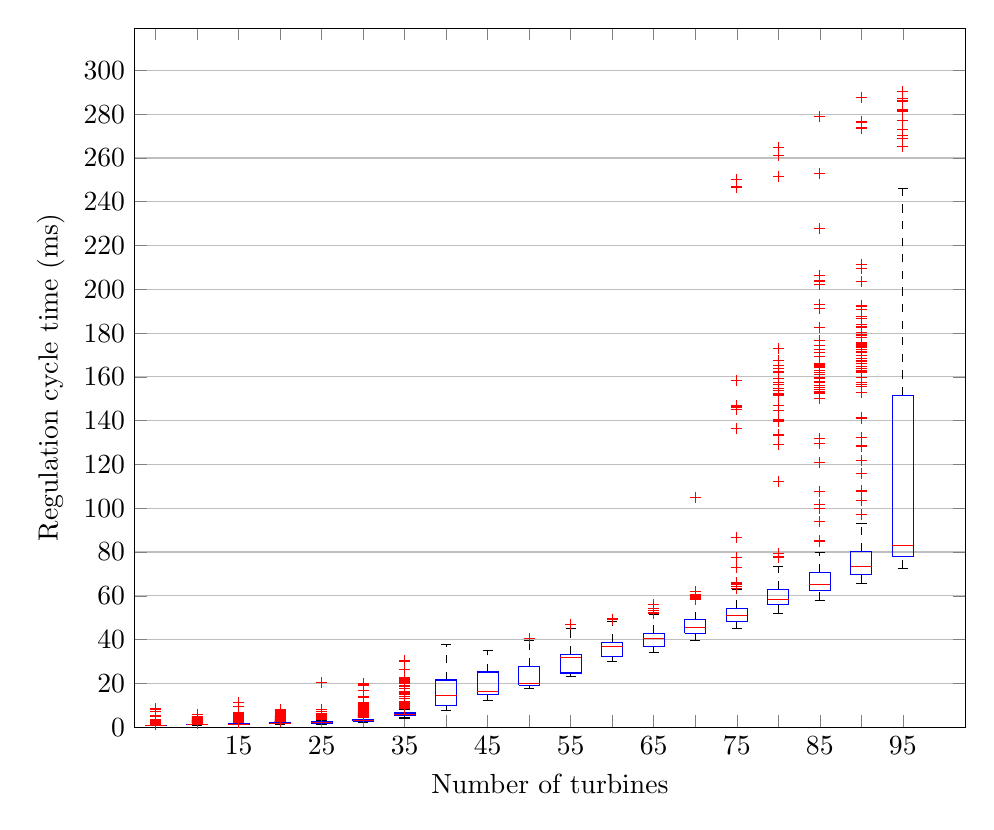
\begin{tikzpicture}

\begin{axis}[%
	width=\resultsPlotWidthScale\textwidth,
	xmin=0.5,
	xmax=20.5,
	xlabel=Number of turbines,
	ylabel=Regulation cycle time (ms),
	xtick={1, 2, 3, 4, 5, 6, 7, 8, 9, 10, 11, 12, 13, 14, 15, 16, 17, 18, 19},
	xticklabels={ , , 15, , 25, , 35, , 45, , 55, , 65, , 75, , 85, , 95},
	ymin=0,
%	ymax=300,
	ymajorgrids=true,
	yminorgrids=true,
	max space between ticks=17.5
]
\addplot [color=black,dashed,forget plot]
  table[row sep=crcr]{%
1	0.955499\\
1	1.156637\\
};
\addplot [color=black,dashed,forget plot]
  table[row sep=crcr]{%
2	1.370008\\
2	1.786582\\
};
\addplot [color=black,dashed,forget plot]
  table[row sep=crcr]{%
3	1.673373\\
3	2.174249\\
};
\addplot [color=black,dashed,forget plot]
  table[row sep=crcr]{%
4	1.958627\\
4	2.487973\\
};
\addplot [color=black,dashed,forget plot]
  table[row sep=crcr]{%
5	2.424964\\
5	3.23762\\
};
\addplot [color=black,dashed,forget plot]
  table[row sep=crcr]{%
6	3.359207\\
6	4.343135\\
};
\addplot [color=black,dashed,forget plot]
  table[row sep=crcr]{%
7	6.472311\\
7	8.243171\\
};
\addplot [color=black,dashed,forget plot]
  table[row sep=crcr]{%
8	21.564196\\
8	37.584364\\
};
\addplot [color=black,dashed,forget plot]
  table[row sep=crcr]{%
9	25.210282\\
9	34.938512\\
};
\addplot [color=black,dashed,forget plot]
  table[row sep=crcr]{%
10	27.678968\\
10	39.521324\\
};
\addplot [color=black,dashed,forget plot]
  table[row sep=crcr]{%
11	33.133063\\
11	45.066276\\
};
\addplot [color=black,dashed,forget plot]
  table[row sep=crcr]{%
12	38.659741\\
12	48.386618\\
};
\addplot [color=black,dashed,forget plot]
  table[row sep=crcr]{%
13	42.692349\\
13	51.64833\\
};
\addplot [color=black,dashed,forget plot]
  table[row sep=crcr]{%
14	48.995592\\
14	58.222076\\
};
\addplot [color=black,dashed,forget plot]
  table[row sep=crcr]{%
15	54.185768\\
15	62.996037\\
};
\addplot [color=black,dashed,forget plot]
  table[row sep=crcr]{%
16	62.88196\\
16	73.366361\\
};
\addplot [color=black,dashed,forget plot]
  table[row sep=crcr]{%
17	70.609667\\
17	79.750216\\
};
\addplot [color=black,dashed,forget plot]
  table[row sep=crcr]{%
18	80.203607\\
18	93.075175\\
};
\addplot [color=black,dashed,forget plot]
  table[row sep=crcr]{%
19	151.608592\\
19	246.076944\\
};
\addplot [color=black,dashed,forget plot]
  table[row sep=crcr]{%
1	0.691463\\
1	0.814662\\
};
\addplot [color=black,dashed,forget plot]
  table[row sep=crcr]{%
2	0.848749\\
2	1.088204\\
};
\addplot [color=black,dashed,forget plot]
  table[row sep=crcr]{%
3	1.082791\\
3	1.330567\\
};
\addplot [color=black,dashed,forget plot]
  table[row sep=crcr]{%
4	1.225531\\
4	1.59823\\
};
\addplot [color=black,dashed,forget plot]
  table[row sep=crcr]{%
5	1.440994\\
5	1.862917\\
};
\addplot [color=black,dashed,forget plot]
  table[row sep=crcr]{%
6	2.148756\\
6	2.694676\\
};
\addplot [color=black,dashed,forget plot]
  table[row sep=crcr]{%
7	4.178016\\
7	5.258074\\
};
\addplot [color=black,dashed,forget plot]
  table[row sep=crcr]{%
8	7.806459\\
8	9.763918\\
};
\addplot [color=black,dashed,forget plot]
  table[row sep=crcr]{%
9	12.116028\\
9	14.873879\\
};
\addplot [color=black,dashed,forget plot]
  table[row sep=crcr]{%
10	17.509834\\
10	19.152298\\
};
\addplot [color=black,dashed,forget plot]
  table[row sep=crcr]{%
11	23.186344\\
11	24.757905\\
};
\addplot [color=black,dashed,forget plot]
  table[row sep=crcr]{%
12	29.984252\\
12	32.129229\\
};
\addplot [color=black,dashed,forget plot]
  table[row sep=crcr]{%
13	33.953182\\
13	36.679471\\
};
\addplot [color=black,dashed,forget plot]
  table[row sep=crcr]{%
14	39.402015\\
14	42.832867\\
};
\addplot [color=black,dashed,forget plot]
  table[row sep=crcr]{%
15	45.162367\\
15	48.235799\\
};
\addplot [color=black,dashed,forget plot]
  table[row sep=crcr]{%
16	51.804628\\
16	55.840494\\
};
\addplot [color=black,dashed,forget plot]
  table[row sep=crcr]{%
17	57.925799\\
17	62.39761\\
};
\addplot [color=black,dashed,forget plot]
  table[row sep=crcr]{%
18	65.7218\\
18	69.72912\\
};
\addplot [color=black,dashed,forget plot]
  table[row sep=crcr]{%
19	72.589561\\
19	77.840082\\
};
\addplot [color=black,solid,forget plot]
  table[row sep=crcr]{%
0.875	1.156637\\
1.125	1.156637\\
};
\addplot [color=black,solid,forget plot]
  table[row sep=crcr]{%
1.875	1.786582\\
2.125	1.786582\\
};
\addplot [color=black,solid,forget plot]
  table[row sep=crcr]{%
2.875	2.174249\\
3.125	2.174249\\
};
\addplot [color=black,solid,forget plot]
  table[row sep=crcr]{%
3.875	2.487973\\
4.125	2.487973\\
};
\addplot [color=black,solid,forget plot]
  table[row sep=crcr]{%
4.875	3.23762\\
5.125	3.23762\\
};
\addplot [color=black,solid,forget plot]
  table[row sep=crcr]{%
5.875	4.343135\\
6.125	4.343135\\
};
\addplot [color=black,solid,forget plot]
  table[row sep=crcr]{%
6.875	8.243171\\
7.125	8.243171\\
};
\addplot [color=black,solid,forget plot]
  table[row sep=crcr]{%
7.875	37.584364\\
8.125	37.584364\\
};
\addplot [color=black,solid,forget plot]
  table[row sep=crcr]{%
8.875	34.938512\\
9.125	34.938512\\
};
\addplot [color=black,solid,forget plot]
  table[row sep=crcr]{%
9.875	39.521324\\
10.125	39.521324\\
};
\addplot [color=black,solid,forget plot]
  table[row sep=crcr]{%
10.875	45.066276\\
11.125	45.066276\\
};
\addplot [color=black,solid,forget plot]
  table[row sep=crcr]{%
11.875	48.386618\\
12.125	48.386618\\
};
\addplot [color=black,solid,forget plot]
  table[row sep=crcr]{%
12.875	51.64833\\
13.125	51.64833\\
};
\addplot [color=black,solid,forget plot]
  table[row sep=crcr]{%
13.875	58.222076\\
14.125	58.222076\\
};
\addplot [color=black,solid,forget plot]
  table[row sep=crcr]{%
14.875	62.996037\\
15.125	62.996037\\
};
\addplot [color=black,solid,forget plot]
  table[row sep=crcr]{%
15.875	73.366361\\
16.125	73.366361\\
};
\addplot [color=black,solid,forget plot]
  table[row sep=crcr]{%
16.875	79.750216\\
17.125	79.750216\\
};
\addplot [color=black,solid,forget plot]
  table[row sep=crcr]{%
17.875	93.075175\\
18.125	93.075175\\
};
\addplot [color=black,solid,forget plot]
  table[row sep=crcr]{%
18.875	246.076944\\
19.125	246.076944\\
};
\addplot [color=black,solid,forget plot]
  table[row sep=crcr]{%
0.875	0.691463\\
1.125	0.691463\\
};
\addplot [color=black,solid,forget plot]
  table[row sep=crcr]{%
1.875	0.848749\\
2.125	0.848749\\
};
\addplot [color=black,solid,forget plot]
  table[row sep=crcr]{%
2.875	1.082791\\
3.125	1.082791\\
};
\addplot [color=black,solid,forget plot]
  table[row sep=crcr]{%
3.875	1.225531\\
4.125	1.225531\\
};
\addplot [color=black,solid,forget plot]
  table[row sep=crcr]{%
4.875	1.440994\\
5.125	1.440994\\
};
\addplot [color=black,solid,forget plot]
  table[row sep=crcr]{%
5.875	2.148756\\
6.125	2.148756\\
};
\addplot [color=black,solid,forget plot]
  table[row sep=crcr]{%
6.875	4.178016\\
7.125	4.178016\\
};
\addplot [color=black,solid,forget plot]
  table[row sep=crcr]{%
7.875	7.806459\\
8.125	7.806459\\
};
\addplot [color=black,solid,forget plot]
  table[row sep=crcr]{%
8.875	12.116028\\
9.125	12.116028\\
};
\addplot [color=black,solid,forget plot]
  table[row sep=crcr]{%
9.875	17.509834\\
10.125	17.509834\\
};
\addplot [color=black,solid,forget plot]
  table[row sep=crcr]{%
10.875	23.186344\\
11.125	23.186344\\
};
\addplot [color=black,solid,forget plot]
  table[row sep=crcr]{%
11.875	29.984252\\
12.125	29.984252\\
};
\addplot [color=black,solid,forget plot]
  table[row sep=crcr]{%
12.875	33.953182\\
13.125	33.953182\\
};
\addplot [color=black,solid,forget plot]
  table[row sep=crcr]{%
13.875	39.402015\\
14.125	39.402015\\
};
\addplot [color=black,solid,forget plot]
  table[row sep=crcr]{%
14.875	45.162367\\
15.125	45.162367\\
};
\addplot [color=black,solid,forget plot]
  table[row sep=crcr]{%
15.875	51.804628\\
16.125	51.804628\\
};
\addplot [color=black,solid,forget plot]
  table[row sep=crcr]{%
16.875	57.925799\\
17.125	57.925799\\
};
\addplot [color=black,solid,forget plot]
  table[row sep=crcr]{%
17.875	65.7218\\
18.125	65.7218\\
};
\addplot [color=black,solid,forget plot]
  table[row sep=crcr]{%
18.875	72.589561\\
19.125	72.589561\\
};
\addplot [color=blue,solid,forget plot]
  table[row sep=crcr]{%
0.75	0.814662\\
0.75	0.955499\\
1.25	0.955499\\
1.25	0.814662\\
0.75	0.814662\\
};
\addplot [color=blue,solid,forget plot]
  table[row sep=crcr]{%
1.75	1.088204\\
1.75	1.370008\\
2.25	1.370008\\
2.25	1.088204\\
1.75	1.088204\\
};
\addplot [color=blue,solid,forget plot]
  table[row sep=crcr]{%
2.75	1.330567\\
2.75	1.673373\\
3.25	1.673373\\
3.25	1.330567\\
2.75	1.330567\\
};
\addplot [color=blue,solid,forget plot]
  table[row sep=crcr]{%
3.75	1.59823\\
3.75	1.958627\\
4.25	1.958627\\
4.25	1.59823\\
3.75	1.59823\\
};
\addplot [color=blue,solid,forget plot]
  table[row sep=crcr]{%
4.75	1.862917\\
4.75	2.424964\\
5.25	2.424964\\
5.25	1.862917\\
4.75	1.862917\\
};
\addplot [color=blue,solid,forget plot]
  table[row sep=crcr]{%
5.75	2.694676\\
5.75	3.359207\\
6.25	3.359207\\
6.25	2.694676\\
5.75	2.694676\\
};
\addplot [color=blue,solid,forget plot]
  table[row sep=crcr]{%
6.75	5.258074\\
6.75	6.472311\\
7.25	6.472311\\
7.25	5.258074\\
6.75	5.258074\\
};
\addplot [color=blue,solid,forget plot]
  table[row sep=crcr]{%
7.75	9.763918\\
7.75	21.564196\\
8.25	21.564196\\
8.25	9.763918\\
7.75	9.763918\\
};
\addplot [color=blue,solid,forget plot]
  table[row sep=crcr]{%
8.75	14.873879\\
8.75	25.210282\\
9.25	25.210282\\
9.25	14.873879\\
8.75	14.873879\\
};
\addplot [color=blue,solid,forget plot]
  table[row sep=crcr]{%
9.75	19.152298\\
9.75	27.678968\\
10.25	27.678968\\
10.25	19.152298\\
9.75	19.152298\\
};
\addplot [color=blue,solid,forget plot]
  table[row sep=crcr]{%
10.75	24.757905\\
10.75	33.133063\\
11.25	33.133063\\
11.25	24.757905\\
10.75	24.757905\\
};
\addplot [color=blue,solid,forget plot]
  table[row sep=crcr]{%
11.75	32.129229\\
11.75	38.659741\\
12.25	38.659741\\
12.25	32.129229\\
11.75	32.129229\\
};
\addplot [color=blue,solid,forget plot]
  table[row sep=crcr]{%
12.75	36.679471\\
12.75	42.692349\\
13.25	42.692349\\
13.25	36.679471\\
12.75	36.679471\\
};
\addplot [color=blue,solid,forget plot]
  table[row sep=crcr]{%
13.75	42.832867\\
13.75	48.995592\\
14.25	48.995592\\
14.25	42.832867\\
13.75	42.832867\\
};
\addplot [color=blue,solid,forget plot]
  table[row sep=crcr]{%
14.75	48.235799\\
14.75	54.185768\\
15.25	54.185768\\
15.25	48.235799\\
14.75	48.235799\\
};
\addplot [color=blue,solid,forget plot]
  table[row sep=crcr]{%
15.75	55.840494\\
15.75	62.88196\\
16.25	62.88196\\
16.25	55.840494\\
15.75	55.840494\\
};
\addplot [color=blue,solid,forget plot]
  table[row sep=crcr]{%
16.75	62.39761\\
16.75	70.609667\\
17.25	70.609667\\
17.25	62.39761\\
16.75	62.39761\\
};
\addplot [color=blue,solid,forget plot]
  table[row sep=crcr]{%
17.75	69.72912\\
17.75	80.203607\\
18.25	80.203607\\
18.25	69.72912\\
17.75	69.72912\\
};
\addplot [color=blue,solid,forget plot]
  table[row sep=crcr]{%
18.75	77.840082\\
18.75	151.608592\\
19.25	151.608592\\
19.25	77.840082\\
18.75	77.840082\\
};
\addplot [color=red,solid,forget plot]
  table[row sep=crcr]{%
0.75	0.874626\\
1.25	0.874626\\
};
\addplot [color=red,solid,forget plot]
  table[row sep=crcr]{%
1.75	1.1775345\\
2.25	1.1775345\\
};
\addplot [color=red,solid,forget plot]
  table[row sep=crcr]{%
2.75	1.4201575\\
3.25	1.4201575\\
};
\addplot [color=red,solid,forget plot]
  table[row sep=crcr]{%
3.75	1.716257\\
4.25	1.716257\\
};
\addplot [color=red,solid,forget plot]
  table[row sep=crcr]{%
4.75	1.9973935\\
5.25	1.9973935\\
};
\addplot [color=red,solid,forget plot]
  table[row sep=crcr]{%
5.75	2.903549\\
6.25	2.903549\\
};
\addplot [color=red,solid,forget plot]
  table[row sep=crcr]{%
6.75	5.5932275\\
7.25	5.5932275\\
};
\addplot [color=red,solid,forget plot]
  table[row sep=crcr]{%
7.75	14.5812775\\
8.25	14.5812775\\
};
\addplot [color=red,solid,forget plot]
  table[row sep=crcr]{%
8.75	16.4337625\\
9.25	16.4337625\\
};
\addplot [color=red,solid,forget plot]
  table[row sep=crcr]{%
9.75	20.091426\\
10.25	20.091426\\
};
\addplot [color=red,solid,forget plot]
  table[row sep=crcr]{%
10.75	31.692363\\
11.25	31.692363\\
};
\addplot [color=red,solid,forget plot]
  table[row sep=crcr]{%
11.75	36.8004425\\
12.25	36.8004425\\
};
\addplot [color=red,solid,forget plot]
  table[row sep=crcr]{%
12.75	40.4086135\\
13.25	40.4086135\\
};
\addplot [color=red,solid,forget plot]
  table[row sep=crcr]{%
13.75	45.333356\\
14.25	45.333356\\
};
\addplot [color=red,solid,forget plot]
  table[row sep=crcr]{%
14.75	50.8482875\\
15.25	50.8482875\\
};
\addplot [color=red,solid,forget plot]
  table[row sep=crcr]{%
15.75	58.49032\\
16.25	58.49032\\
};
\addplot [color=red,solid,forget plot]
  table[row sep=crcr]{%
16.75	65.293539\\
17.25	65.293539\\
};
\addplot [color=red,solid,forget plot]
  table[row sep=crcr]{%
17.75	73.479706\\
18.25	73.479706\\
};
\addplot [color=red,solid,forget plot]
  table[row sep=crcr]{%
18.75	82.948313\\
19.25	82.948313\\
};
\addplot [color=blue,only marks,mark=+,mark options={solid,draw=red},forget plot]
  table[row sep=crcr]{%
1	1.176103\\
1	1.178509\\
1	1.193344\\
1	1.20704\\
1	1.214954\\
1	1.221493\\
1	1.245021\\
1	1.316445\\
1	1.327208\\
1	1.524131\\
1	1.524274\\
1	1.543741\\
1	1.902597\\
1	2.169802\\
1	2.307744\\
1	2.476555\\
1	2.709384\\
1	2.981451\\
1	3.140805\\
1	3.283617\\
1	4.963499\\
1	5.363371\\
1	7.190786\\
1	8.30093\\
};
\addplot [color=blue,only marks,mark=+,mark options={solid,draw=red},forget plot]
  table[row sep=crcr]{%
2	1.793523\\
2	1.845619\\
2	1.848076\\
2	1.933673\\
2	1.99282\\
2	2.051408\\
2	2.120934\\
2	2.151493\\
2	2.249679\\
2	2.262758\\
2	2.300418\\
2	2.368791\\
2	2.401617\\
2	2.481835\\
2	2.53602\\
2	2.548682\\
2	2.576888\\
2	2.597632\\
2	2.677461\\
2	2.723364\\
2	2.740618\\
2	2.774466\\
2	2.867248\\
2	2.899936\\
2	2.944661\\
2	2.965056\\
2	2.96526\\
2	2.981629\\
2	3.089347\\
2	3.131373\\
2	3.180755\\
2	3.306036\\
2	3.332826\\
2	3.449926\\
2	3.489132\\
2	3.672439\\
2	3.706892\\
2	3.749078\\
2	3.877362\\
2	4.023028\\
2	4.389004\\
2	4.398121\\
2	4.401876\\
2	4.678904\\
2	4.779742\\
2	4.918733\\
2	5.075662\\
2	5.601809\\
};
\addplot [color=blue,only marks,mark=+,mark options={solid,draw=red},forget plot]
  table[row sep=crcr]{%
3	2.192261\\
3	2.222847\\
3	2.223433\\
3	2.239635\\
3	2.245748\\
3	2.337855\\
3	2.564155\\
3	2.566424\\
3	2.568352\\
3	2.629852\\
3	2.652528\\
3	2.703118\\
3	2.733534\\
3	2.764757\\
3	2.783863\\
3	2.828118\\
3	2.846928\\
3	2.984215\\
3	3.051839\\
3	3.071094\\
3	3.081963\\
3	3.230031\\
3	3.352067\\
3	3.690988\\
3	3.70011\\
3	3.71423\\
3	4.081016\\
3	4.251259\\
3	4.299668\\
3	4.317077\\
3	4.378226\\
3	4.655414\\
3	4.800068\\
3	5.335757\\
3	5.455589\\
3	5.596238\\
3	5.710081\\
3	5.790715\\
3	6.364993\\
3	6.679123\\
3	9.543143\\
3	11.395216\\
};
\addplot [color=blue,only marks,mark=+,mark options={solid,draw=red},forget plot]
  table[row sep=crcr]{%
4	2.503863\\
4	2.506996\\
4	2.518698\\
4	2.519083\\
4	2.524849\\
4	2.538949\\
4	2.539779\\
4	2.543708\\
4	2.590436\\
4	2.612976\\
4	2.624723\\
4	2.639969\\
4	2.692657\\
4	2.701875\\
4	2.702706\\
4	2.776353\\
4	2.834106\\
4	2.874534\\
4	2.903889\\
4	2.921809\\
4	2.947651\\
4	3.016038\\
4	3.18633\\
4	3.256435\\
4	3.289407\\
4	3.470499\\
4	3.523172\\
4	3.573076\\
4	3.614098\\
4	3.621255\\
4	3.757607\\
4	3.911986\\
4	4.033259\\
4	4.073237\\
4	4.338524\\
4	4.399647\\
4	4.630443\\
4	4.664954\\
4	4.779427\\
4	4.906645\\
4	4.925404\\
4	5.040655\\
4	5.079302\\
4	5.373808\\
4	6.030455\\
4	6.328306\\
4	6.626284\\
4	6.999776\\
4	7.221142\\
4	7.451491\\
4	7.916905\\
};
\addplot [color=blue,only marks,mark=+,mark options={solid,draw=red},forget plot]
  table[row sep=crcr]{%
5	3.320071\\
5	3.377586\\
5	3.423061\\
5	3.427332\\
5	3.53449\\
5	3.546939\\
5	3.746197\\
5	3.765826\\
5	3.782267\\
5	3.787644\\
5	3.824862\\
5	3.893861\\
5	3.959252\\
5	4.037436\\
5	4.097061\\
5	4.125631\\
5	4.133696\\
5	4.138075\\
5	4.147994\\
5	4.176374\\
5	4.421668\\
5	4.513637\\
5	4.616056\\
5	4.635814\\
5	4.753148\\
5	5.167944\\
5	5.19975\\
5	5.420932\\
5	5.455067\\
5	5.665121\\
5	5.721665\\
5	5.83401\\
5	5.87468\\
5	5.89412\\
5	5.921696\\
5	6.057049\\
5	6.131888\\
5	6.296973\\
5	6.321923\\
5	6.343328\\
5	7.090603\\
5	8.26168\\
5	20.243534\\
};
\addplot [color=blue,only marks,mark=+,mark options={solid,draw=red},forget plot]
  table[row sep=crcr]{%
6	4.495225\\
6	4.498673\\
6	4.498827\\
6	4.563186\\
6	4.587355\\
6	4.754654\\
6	5.009052\\
6	5.021732\\
6	5.102506\\
6	5.158721\\
6	5.167734\\
6	5.198709\\
6	5.23857\\
6	5.3746\\
6	5.400768\\
6	5.471458\\
6	5.487853\\
6	5.732529\\
6	5.758585\\
6	5.785591\\
6	5.904012\\
6	6.088597\\
6	6.13559\\
6	6.338497\\
6	6.607769\\
6	6.707598\\
6	6.847774\\
6	6.863557\\
6	6.923896\\
6	6.932131\\
6	6.966114\\
6	7.246241\\
6	7.552089\\
6	7.637072\\
6	8.035988\\
6	8.318994\\
6	8.349444\\
6	8.519427\\
6	8.777099\\
6	9.338181\\
6	9.720935\\
6	9.898789\\
6	10.188432\\
6	10.358991\\
6	10.590425\\
6	11.26527\\
6	13.649585\\
6	13.917339\\
6	16.898115\\
6	19.216894\\
6	19.71008\\
};
\addplot [color=blue,only marks,mark=+,mark options={solid,draw=red},forget plot]
  table[row sep=crcr]{%
7	8.35779\\
7	8.415277\\
7	8.473364\\
7	8.504532\\
7	8.506126\\
7	8.519745\\
7	8.553583\\
7	8.5815\\
7	8.663745\\
7	8.678187\\
7	8.683617\\
7	8.78386\\
7	8.849726\\
7	8.950628\\
7	8.987027\\
7	8.992308\\
7	9.120563\\
7	9.207595\\
7	9.23472\\
7	9.345101\\
7	9.398249\\
7	9.423573\\
7	9.439464\\
7	9.486276\\
7	9.521467\\
7	9.580156\\
7	9.590542\\
7	9.629696\\
7	9.657168\\
7	9.679038\\
7	9.768644\\
7	9.773259\\
7	9.820831\\
7	9.965677\\
7	10.269888\\
7	10.302693\\
7	10.323261\\
7	10.420508\\
7	10.88144\\
7	10.912448\\
7	10.912924\\
7	10.922096\\
7	11.006882\\
7	11.222083\\
7	11.30686\\
7	11.547859\\
7	13.009371\\
7	14.092999\\
7	14.86172\\
7	15.293268\\
7	15.773637\\
7	16.071576\\
7	17.524366\\
7	18.635734\\
7	18.86347\\
7	18.884021\\
7	19.925684\\
7	20.211662\\
7	20.368998\\
7	20.490724\\
7	20.838327\\
7	20.957185\\
7	21.053338\\
7	21.479073\\
7	21.720464\\
7	21.952807\\
7	22.450527\\
7	26.466628\\
7	29.810133\\
7	29.924012\\
7	30.656609\\
};
\addplot [color=blue,only marks,mark=+,mark options={solid,draw=red},forget plot]
  table[row sep=crcr]{%
nan	nan\\
};
\addplot [color=blue,only marks,mark=+,mark options={solid,draw=red},forget plot]
  table[row sep=crcr]{%
nan	nan\\
};
\addplot [color=blue,only marks,mark=+,mark options={solid,draw=red},forget plot]
  table[row sep=crcr]{%
10	40.572149\\
};
\addplot [color=blue,only marks,mark=+,mark options={solid,draw=red},forget plot]
  table[row sep=crcr]{%
11	46.841843\\
};
\addplot [color=blue,only marks,mark=+,mark options={solid,draw=red},forget plot]
  table[row sep=crcr]{%
12	49.32547\\
12	49.39728\\
};
\addplot [color=blue,only marks,mark=+,mark options={solid,draw=red},forget plot]
  table[row sep=crcr]{%
13	51.734931\\
13	52.263042\\
13	52.479868\\
13	53.346653\\
13	53.380803\\
13	54.235959\\
13	56.218855\\
};
\addplot [color=blue,only marks,mark=+,mark options={solid,draw=red},forget plot]
  table[row sep=crcr]{%
14	58.24263\\
14	58.359494\\
14	58.779699\\
14	59.255721\\
14	59.797221\\
14	59.956779\\
14	59.989437\\
14	60.023581\\
14	60.358906\\
14	60.684411\\
14	61.858036\\
14	104.953184\\
};
\addplot [color=blue,only marks,mark=+,mark options={solid,draw=red},forget plot]
  table[row sep=crcr]{%
15	63.495834\\
15	64.370846\\
15	65.078212\\
15	65.674834\\
15	65.803883\\
15	65.835327\\
15	66.021914\\
15	66.103339\\
15	73.001122\\
15	77.636315\\
15	86.826142\\
15	136.487634\\
15	145.283402\\
15	146.099428\\
15	146.233285\\
15	146.323243\\
15	146.921872\\
15	158.423312\\
15	246.362832\\
15	246.722952\\
15	250.200229\\
};
\addplot [color=blue,only marks,mark=+,mark options={solid,draw=red},forget plot]
  table[row sep=crcr]{%
16	77.720929\\
16	79.177628\\
16	112.408851\\
16	128.969515\\
16	133.462981\\
16	139.858548\\
16	140.725977\\
16	144.612062\\
16	146.817379\\
16	151.383076\\
16	151.881108\\
16	151.922485\\
16	152.242982\\
16	153.688064\\
16	154.509165\\
16	156.475983\\
16	157.507242\\
16	159.324566\\
16	162.256717\\
16	164.015403\\
16	165.32339\\
16	167.323423\\
16	172.786236\\
16	251.349021\\
16	261.289044\\
16	264.827819\\
};
\addplot [color=blue,only marks,mark=+,mark options={solid,draw=red},forget plot]
  table[row sep=crcr]{%
17	85.033259\\
17	85.168934\\
17	93.984073\\
17	99.985429\\
17	101.754141\\
17	107.502865\\
17	120.708505\\
17	129.533025\\
17	131.685524\\
17	150.07707\\
17	152.531279\\
17	152.848707\\
17	153.515564\\
17	154.184764\\
17	154.425517\\
17	155.223244\\
17	155.325952\\
17	156.040595\\
17	157.51096\\
17	157.745791\\
17	157.763823\\
17	157.78978\\
17	159.313071\\
17	159.792905\\
17	161.075164\\
17	161.182074\\
17	161.201118\\
17	162.147412\\
17	163.084965\\
17	164.144737\\
17	164.432633\\
17	164.531559\\
17	165.276971\\
17	165.915944\\
17	166.24057\\
17	169.122972\\
17	170.956902\\
17	172.574969\\
17	174.203491\\
17	174.230232\\
17	176.682499\\
17	182.438894\\
17	191.366639\\
17	192.967176\\
17	202.370675\\
17	203.807066\\
17	206.229644\\
17	227.845875\\
17	252.720361\\
17	278.866888\\
};
\addplot [color=blue,only marks,mark=+,mark options={solid,draw=red},forget plot]
  table[row sep=crcr]{%
18	97.320739\\
18	103.607594\\
18	107.896473\\
18	116.060945\\
18	121.809576\\
18	128.452211\\
18	132.177856\\
18	141.230189\\
18	152.923783\\
18	155.730984\\
18	156.691553\\
18	157.523825\\
18	159.835414\\
18	159.897403\\
18	161.962464\\
18	162.510937\\
18	162.565594\\
18	163.007536\\
18	163.988911\\
18	164.705291\\
18	165.959133\\
18	167.195639\\
18	167.26318\\
18	167.489415\\
18	167.573509\\
18	168.458682\\
18	169.70467\\
18	171.087881\\
18	171.523672\\
18	171.531448\\
18	171.659207\\
18	172.561978\\
18	172.716008\\
18	173.315331\\
18	173.869469\\
18	174.119127\\
18	174.807872\\
18	175.47089\\
18	178.054177\\
18	178.925643\\
18	179.325541\\
18	180.261783\\
18	182.703061\\
18	183.168246\\
18	183.804264\\
18	186.546645\\
18	187.398376\\
18	190.73619\\
18	192.117568\\
18	192.334748\\
18	192.687149\\
18	203.621105\\
18	209.714732\\
18	211.529157\\
18	273.591922\\
18	274.074762\\
18	276.443283\\
18	287.542878\\
};
\addplot [color=blue,only marks,mark=+,mark options={solid,draw=red},forget plot]
  table[row sep=crcr]{%
19	265.296814\\
19	268.749173\\
19	270.245766\\
19	273.069504\\
19	277.122711\\
19	281.054363\\
19	281.926684\\
19	282.148412\\
19	285.594887\\
19	286.16293\\
19	287.331069\\
19	290.243704\\
};
\node[above, align=center, inner sep=0mm, text=black]
at (axis cs:9.13684210526316,-12,0) {1};
\node[above, align=center, inner sep=0mm, text=black]
at (axis cs:27.4105263157895,-12,0) {2};
\node[above, align=center, inner sep=0mm, text=black]
at (axis cs:45.6842105263158,-12,0) {3};
\node[above, align=center, inner sep=0mm, text=black]
at (axis cs:63.9578947368421,-12,0) {4};
\node[above, align=center, inner sep=0mm, text=black]
at (axis cs:82.2315789473684,-12,0) {5};
\node[above, align=center, inner sep=0mm, text=black]
at (axis cs:100.505263157895,-12,0) {6};
\node[above, align=center, inner sep=0mm, text=black]
at (axis cs:118.778947368421,-12,0) {7};
\node[above, align=center, inner sep=0mm, text=black]
at (axis cs:137.052631578947,-12,0) {8};
\node[above, align=center, inner sep=0mm, text=black]
at (axis cs:155.326315789474,-12,0) {9};
\node[above, align=center, inner sep=0mm, text=black]
at (axis cs:173.6,-12,0) {10};
\node[above, align=center, inner sep=0mm, text=black]
at (axis cs:191.873684210526,-12,0) {11};
\node[above, align=center, inner sep=0mm, text=black]
at (axis cs:210.147368421053,-12,0) {12};
\node[above, align=center, inner sep=0mm, text=black]
at (axis cs:228.421052631579,-12,0) {13};
\node[above, align=center, inner sep=0mm, text=black]
at (axis cs:246.694736842105,-12,0) {14};
\node[above, align=center, inner sep=0mm, text=black]
at (axis cs:264.968421052632,-12,0) {15};
\node[above, align=center, inner sep=0mm, text=black]
at (axis cs:283.242105263158,-12,0) {16};
\node[above, align=center, inner sep=0mm, text=black]
at (axis cs:301.515789473684,-12,0) {17};
\node[above, align=center, inner sep=0mm, text=black]
at (axis cs:319.789473684211,-12,0) {18};
\node[above, align=center, inner sep=0mm, text=black]
at (axis cs:338.063157894737,-12,0) {19};
\end{axis}
\end{tikzpicture}%
	\caption{Centralized solution variable number of turbines}
	\label{fig:exp:cen:turbines}
\end{figure}

\Cref{fig:exp:cen:turbines} shows how the number of turbines influence the regulation cycle time of the centralized solution.
For every number of turbines 450 data points have been sampled. The reason for the limited amount of samples is that when running the experiment with 95 turbines the test setup is reaching it's limits. Data transfer speeds of up to 75 Mbit/s was observed. Since the maximum theoretical data transfer speed of the test setup is 100 Mbit/s it is reasonable to assume that a number of packages have been lost due to congestion. Thus, the experiment for 95 turbines only managed to log 450 data samples within the given experiment time. In order to create a boxplot with comparable values the sample set for each number of turbines was reduced to the 450 first points.
The limited amount of data samples account for the "holes" between outlier values. With more data samples these holes would be filled such that outliers are more evenly distributed from the top whisker to the most extreme outlier.

The median values from 5 to 30 turbines is increasing slightly. From 35 turbines and onward the median is linearly increasing.
From 75 turbines onward the outliers take on increasingly extreme values, which is when the test setup starts to be unable to handle the number of packages sent in the network. Results from 75 turbines and onward should be disregarded.

\subsection{Discussion}
The test results from the centralized solution presented in \cref{fig:exp:cen:turbines} shows how adding turbines increases the regulation cycle time. From 5 to 30 turbines the regulation time of the centralized solution increase slowly. After 35 turbines the increase in regulation cycle time becomes steeper. For every 15 turbines added the regulation cycle time increases with approximately $25 ms$. The relation between regulation cycle time and the number of turbines is caused by the direct impact the number of turbines have on the regulation cycle. The Park Pilot of the centralized solution must use additional time on querying each added turbine as well as wait for their individual reply before performing the regulation algorithm. Thus the scalability of the centralized solution is linear with a factor of approximately $25 / 15 = 1.667$ ms added regulation cycle time per added turbine.
The outliers of \cref{fig:exp:cen:turbines} is distributed fairly close around the medains from 5 to 70 turbines. From 75 turbines on the outliers quadruple in regulation cycle time which is a sign that the test setup has reached it's limits. The heavily increased regulation cycle time for the outliers is a result of lost or delayed network packages forcing the Park Pilot to wait for a retransmission of turbine state before the regulation cycle can be completed.

\subsubsection{Comparison of the decentralized solution and the centralized solution}
\label{sec:comp:decentralizedVScentralized}
The decentralized solution and the centralized solution is built with a very different architecture. This is reflected in the difference in the way the two solutions scale with the number of turbines. Looking at the figures for regulation cycle time in relation to the number of turbines for the decentralized and the centralized solution respectively we see that the figures reveals different trends.

The scalability of the centralized solution is linear with a factor of approximately $1.667$ ms added to regulation cycle time per turbine added to the system.
The scalability of the decentralized solution, as described in \cref{sec:disc:turbinesVScycletime}, is small enough that it is indistinguishable from other factors in our test data and therefore we cannot calculate it. Thus the scalability of the decentralized solution is close to constant. This great improvement in scalability comes with a trade off in terms of cache reads. Adding additional turbines to the decentralized solution the number of cache reads increases with a factor of $0.033$ extra cache reads per added turbine which is still an improvement compared to the scale factor of the centralized solution. Arguably comparing the scalability of the number of cache reads in the decentralized solution with the scalability of the regulation cycle in the centralized solution is not a viable way to compare the scalability of the two solutions, but comparing the scalability of the regulation cycle of both solutions will not be a fair comparison either since the improvements in scalability of the decentralized solution comes at the price of increased numbers of cache reads.

\subsubsection{Comparison of the decentralized solution and the current Siemens system}
This section address the \ref{PS:Q:Scalability} problem of \cref{sec:problemStatement}.
Comparing the decentralized solution and the current Siemens system directly is impossible given the differences in environment and architecture. Introducing a centralized solution is an attempt to bridge this gap. By comparing the decentralized solution to the centralized solution and measuring the improvements/demotions we can transfer these measures to the current Siemens system and an imagined decentralized implementation of the current Siemens system.

Looking at \cref{sec:comp:decentralizedVScentralized} there is an advantage in scalability when running a decentralized solution compared to a centralized. This is underlined by the improvement in regulation cycle time of the decentralized solution compared to the centralized solution. The improvement of the scalability of the regulation cycle time comes at the price of the chance that the regulation may be performed on cached data.

Decentralizing the current Siemens system will enable improvements on other areas than regulation cycle time. By removing the centralized Park Pilots and the Wind Power Supervisor of the current Siemens solution the regulation of turbines, data storage and external communication of these must be decentralized and placed in the turbines themselves. This requires the use of software components that are able to handle regulation of turbines, data storage and external communication in a fashion such that if a turbine failure occurs other turbines can increase production to make up for the missing power production, provide access to the data collected on the failing turbine and handle external communication the failing turbine may have been handling. This increases the availability of the wind farm compared to the current Siemens system.


